\documentclass[grado3]{LEMA-Tikz-IM}
\begin{document}

\graphicspath{{../../tikz-source/}}

\def\figScale{0.72} % common scale for all tikz figs in cells (so that dots have the same size)

% stop hyphenation
\hyphenpenalty=10000
\tolerance=1000

\begin{tikzpicture}
\matrix[tablaVertical, % ver def en LEMA-Tikz-IM.sty
        row 1/.append style={nodes={minimum height=9ex}},
        row 2/.append style={nodes={minimum height=24ex}},
        row 3/.append style={nodes={minimum height=22ex}},
        row 4/.append style={nodes={minimum height=17ex}},
        row 5/.append style={nodes={minimum height=18ex}},
        column 1/.append style={nodes={text width = 20ex}},
        column 2/.append style={nodes={text width = 15ex}},
        column 3/.append style={nodes={text width = 15ex}},
        column 4/.append style={nodes={text width = 14ex}},
    ] (myTable) {
        % Header Row 
        {situación} & dibujo o diagrama & {ecuación de multiplicación}& {ecuación de división}\\\\
        % contenido tabla para statement y BLM
        % fila 1
La familia de Elena compra 18 aguacates en el mercado agrícola. Hay 3 aguacates en cada bolsa. 
& \node {
\includegraphics[scale=\figScale]{tikz-file-3-4-B-131870.pdf}};
&    
&  $18 \div 3 = \underline{\hspace{0.7 cm}}$
\\% 
% fila 2
Andre ve 25 tomates. Están en 5 racimos. Cada racimo tiene el mismo número de tomates. 
&  
& $5 \times {?} = 25$ 
& $25 \div 5 = {?}$ 
\\% 
% fila 3
Lin pide 6 buñuelos de banano. Los buñuelos se sirven en 2 platos y cada plato tiene el mismo número de buñuelos. 
& \node {
\includegraphics[scale=\figScale]{tikz-file-3-4-B-131871.pdf}};
& $2 \times{ ?} = 6$ 
&   
\\%
% fila 4
% 
& \node {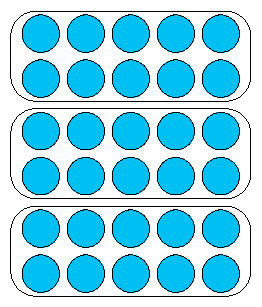
\includegraphics[scale=\figScale]{tikz-file-3-4-B-131872.pdf}};
& $\underline{\hspace{0.7 cm}} \times 10 = 30$ 
&  $30 \div 10 = \underline{\hspace{0.7 cm}}$ \\
  };

\end{tikzpicture}


\end{document}